\documentclass[thesis.tex]{subfiles}

\newcommand{\inner}[2]{\left<#1, #2\right>}
\newcommand{\alemap}{\ensuremath{\mathcal{A}}}
\newcommand{\dt}{\ensuremath{\Delta t}}
\newcommand{\pexp}{\ensuremath{\frac{2\gamma}{\left(\gamma-1\right)}}}
\newcommand{\aleX}{\ensuremath{\mathcal{X}}}
\newcommand{\Ah}[1]{\ensuremath{\vb{#1}^{n+1}_h}}
\newcommand{\Ahn}[1]{\ensuremath{\vb{#1}^{n}_h}}

\newcommand{\rbV}{\ensuremath{\mathbb{V}}}
\newcommand{\rbVT}{\ensuremath{\rbV^T}}
\newcommand{\epspod}{\ensuremath{\varepsilon_\text{POD}}}

\begin{document}

\section*{List of Symbols}
\addcontentsline{toc}{section}{List of Symbols}

\begin{table}[h]        
    \begin{tabular}{cl}
        % Symbol & Description \\
        % \midrule
        $t$ & time coordinate \\
        $x$ & space coordinate in the physical domain \\
        $\aleX$ & space coordinate in a fixed reference domain \\
        $\alemap$ & Arbitrary Lagrangian Eulerian map \\
        $d$ & mesh displacement \\
        $w_m$ & mesh velocity \\
        $J$ & Jacobian matrix \\
        $J_\alemap$ & Jacobian transformation (matrix determinant) \\
        $L_0$ & initial piston length \\
        $L$ & piston movement in time \\
        $u$ & flow velocity \\
        $\hat{u}$ & flow velocity for the homogeneous problem \\
        $u_h$ & flow velocity finite element representation \\ 
        $g$ & Dirichlet boundary lifting \\ 
        $p$ & pressure \\
        $\rho$ & density \\
        $\gamma$ & specific heat ratio \\
        $MD$ & mass defect in time (numerical integration) \\
        $\varepsilon$ & artificial viscosity value \\
        $\varepsilon_{POD}$ & POD approximation error \\
        $u_p$ & piston mach number \\
        $a_0$ & reference speed of sound \\
        $p_0$ & reference pressure \\
        $\rho_0$ & reference density \\
        $\delta$ & piston displacement from rest \\
        $\omega$ & piston oscillating frequency  \\
        $c$ & dimensionless convection velocity \\
        $b_0$ & dimensionless constant convection coefficient \\
        $b_L$ & dimensionless piston boundary condition \\
        $\mathcal{F}$ & Gaussian bell \\
        $x_c$ & Gaussian bell center \\
        $\sigma_c$ & Gaussian bell dispersion factor \\
        $y_c$ & Gaussian bell scaling factor \\
        $N_h$ & number of finite element degrees of freedom \\ 
        $N$ & number of reduced basis degrees of freedom \\ 
        $V_h$ & space of Lagrangian functions\\ 
        $V_N$ & space of RB solution modes\\ 
        $\varphi_i$ & Lagrangian finite element basis function \\ 
        $\psi_i$ & RB solution modes \\
        $A_{h,q}$ & algebraic operator modes (collateral basis)\\ 
    \end{tabular}
\end{table}

\newpage 
\section{Introduction}
When a painter sets out to paint, she will probably use most of the available basic colours.
However, if she knew beforehand that she was only going to paint landscapes, 
she would fare well with a farsighted palette: greens, browns, blues, whites, etc.
Such is the nature of Reduced Order Models, 
to find a subset among the combinations of basic colours 
to represent the solution to the problem of interest.

In the context of this work, 
the basic colours are the classical mathematical Lagrangian finite element basis functions: 
generic, piecewise, with local support, able to represent most functions of interest.
Instead, the landscape palette will be ad-hoc:
problem-dependent functions with global support, 
good at capturing details only specific to landscapes.

Additionally, she will not need all sorts of brushes, 
simply the ones with the right thickness and width for mountains, trees and hills.
The brushes represent the algebraic operators that arise from the finite element discretization.
As with the colours, we can find a subset of combinations of brushes that suit our problem.
That is, we can find a basis for each algebraic operator to build them efficiently.

Finally, since she is a vanguard painter, the domain of our problem, her canvas, 
will be allowed to change in time as she paints.
The landscape colours and brushes we select will need to take this into account.

So far with metaphors.

\subsection{Purpose and Layout}
We are going to build and certify an
{hyper reduced order model} 
for a one-dimensional parametrized piston problem, 
whose movement is prescribed.
The adjective \mbox{\textit{hyper}}\footnote{
    Word-forming element meaning "over, above, beyond", 
    and often implying "exceedingly, to excess".
    From Greek \textit{hyper} (prep. and adv.) 
    "over, beyond, overmuch, above measure".
} is present because 
a collateral basis will be created for each algebraic operator,
on top of the one created for the solution space.
The model PDE, the boundary conditions and the geometrical configuration will be parametrized.

This work extends \cite{Santo_Manzoni_2019,2015_efficientModelReductionParametrizedSystemsMatrixDeim_Negri}
(albeit for a simpler PDE), 
which introduced the MDEIM technique for parametrized domains, whose mesh remained fixed in time.

\subsubsection{Thesis Goal}
Physical problems with moving meshes may require 
the introduction of a transformation in the weak form,
to translate the PDE defined in a deforming space into a fixed, 
numerical grid, as shown in Figure~\ref{fig:jacobianTransformation}.
\begin{figure}[h]
    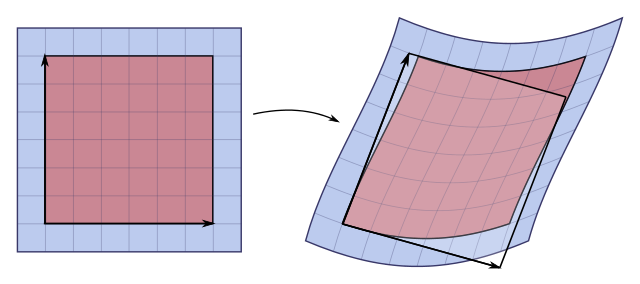
\includegraphics[width=\columnwidth]{research_project/piston/figures/Jacobian_determinant_and_distortion.png}
    \caption{Numerical fixed grid to the left, physical moving mesh to the right.
    The Jacobian determinant establishes the connection between 
    the evalaution of an integral over the red square.
    Figure from \cite{jacobianTransformation}.}
    \label{fig:jacobianTransformation}
\end{figure}

This transformation can take many names, 
such as generalized transformation, 
mapping,
boundary-conforming coordinate transformation,
etc.
% mapping},
It usually involves the computation of a Jacobian matrix $J$,
whose determinant plays an important role in the aforementioned transformation.

The elements of the Jacobian matrix might be known explicitly,
if the deformation is known analytically and the domain is sufficiently simple.
However, if the domain takes arbitrary shapes 
(likely for real-life problems in higher dimensions than one),
or we are dealing with an FSI problem (where the deformation is part of the solution),
it is quite possible that we have to compute the Jacobian transformation numerically.
This is likely to be an undesirable situation, 
for the physical weak form will become contaminated with additional terms, 
making it more cumbersome to implement and deal with\footnote{
    The discretization will not be formulated for the original variable~$\phi$,
    but rather for its distorted counterpart~$J \phi$.
    },
as well as the inevitable overhead in computational costs.

This overhead created by the Jacobian is likely to permeate to the Reduced Order Model (ROM),
for in the context of Finite Elements, ROMs are often built as a system with the same algebraic structure
as the departing Full Order Model (FOM),
albeit with smaller matrices and vectors. 
It might even be the case that we cannot completely uncouple the ROM from the FOM, 
if the problem is complex enough, or that we need satellite ROMs to compute the Jacobian matrix efficiently.

Hence, to avoid all of the previous, 
we are going to track down a formulation which allows us to remain in the physical domain, 
whilst maintaining a perfect \textit{offline-online} decomposition,
making our reduction scheme reach the maximum of its efficiency capacities.

\subsubsection{Document Layout}
The layout of the document is as follows:
\begin{itemize}
    \item in Section~\ref{sec:fom_definition} we define the Full Order Model, that is, 
    the model PDE and its boundary conditions, 
    mesh deformation and the associated Arbitrary Lagrangian Eulerian (ALE) formulation
    in the physical domain,
    both at the continuous and discrete levels;
    \item in Section~\ref{sec:rom_definition} we explain the details of the reduction scheme, 
    along with the system approximation technique (M)DEIM;
    \item in Section~\ref{sec:fom_calibration} we analyze the FOM discretization, 
    and show convergence figures and solutions for the moving piston for different parametrizations;
    \item finally, in Section~\ref{sec:results_and_certification} we present reduction results
    and certify the reduction scheme with an efficient a posteriori error estimators obtained via model truncation.
\end{itemize}
Before all that, we frame our work within the current body of knowledge 
with a short literature review.
Additional references will be cited within the body of the document, 
where their appearence is more accurate and helpful.  

\subsection{Literature Review}
%% Lab Report for EEET2493_labreport_template.tex
%% V1.0
%% 2019/01/16
%% This is the template for a Lab report following an IEEE paper. Modified by Francisco Tovar after Michael Sheel original document.


%% This is a skeleton file demonstrating the use of IEEEtran.cls
%% (requires IEEEtran.cls version 1.8b or later) with an IEEE
%% journal paper.
%%
%% Support sites:
%% http://www.michaelshell.org/tex/ieeetran/
%% http://www.ctan.org/pkg/ieeetran
%% and
%% http://www.ieee.org/

%%*************************************************************************
%% Legal Notice:
%% This code is offered as-is without any warranty either expressed or
%% implied; without even the implied warranty of MERCHANTABILITY or
%% FITNESS FOR A PARTICULAR PURPOSE! 
%% User assumes all risk.
%% In no event shall the IEEE or any contributor to this code be liable for
%% any damages or losses, including, but not limited to, incidental,
%% consequential, or any other damages, resulting from the use or misuse
%% of any information contained here.
%%
%% All comments are the opinions of their respective authors and are not
%% necessarily endorsed by the IEEE.
%%
%% This work is distributed under the LaTeX Project Public License (LPPL)
%% ( http://www.latex-project.org/ ) version 1.3, and may be freely used,
%% distributed and modified. A copy of the LPPL, version 1.3, is included
%% in the base LaTeX documentation of all distributions of LaTeX released
%% 2003/12/01 or later.
%% Retain all contribution notices and credits.
%% ** Modified files should be clearly indicated as such, including  **
%% ** renaming them and changing author support contact information. **
%%*************************************************************************

% \documentclass[a4paper, technote, compsoc]{IEEEtran}
\documentclass[literature_review.tex]{subfiles}

\begin{document}

\section{Introduction}

% Theoretical
% A literature review is often the foundation for a theoretical framework. 
% You can use it to discuss various theories, models, and definitions of key concepts.
% You might argue for the relevance of a specific theoretical approach, 
% or combine various theoretical concepts to create a framework for your research.
In the following we present the relevant literature used in this work.
% We have preferred to group references by conceptual blocks, 
% and towards the end bridge all of them together.
We have used mainly two types of papers: 
methodology and applications.
The former present a numerical method or formulation 
which we use, 
the latter make use of it in a different or similar context as we do.
We were especially interested in the applications to see how
previous works dealt with inhomogeneous boundary conditions,
on which more later on in the work and the review.

\subsubsection{Burgers Terms and Piston Models}
Regarding the target PDE to work with, we decided upon several constraints:
it had to be one-dimensional (to ease implementation), 
contain non-trivial terms (to make the problem interesting),
and be physically sound (to validate the outcome).

The first two constraints are satisfied by an advection equation with 
a nonlinear Burgers-like convective term.
Burgers equation showed up in the gas dynamics literature several decades ago
\cite{BURGERS1948171,
moran_shen_1966,
1969nonlinearWavePropagationInARelaxingGas,
1951_quasiLinearParabolicEquationOcuringAerodynamics},
for which under controlled conditions 
a range of implicit analytical solutions exist \cite{1972_TableSolutionsBurgers},
including moving domains \cite{2000_burgersMovingDomainAnalytical}.

Nevertheless, most of the mentioned solutions are either asymptotic,
computed in a moving frame of reference\footnote{
    It is important to make the distinction between a \textit{moving domain}
    and a \textit{moving coordinate system}.
    The former is deformed around the same neighborhood in space,
    whilst the latter is displacing itself across space.
}, 
or defined for an infinite or fixed domain.
Additionally, to obtain the results integral formulations have to be solved 
(the simple solutions are only defined for fixed domains).
Hence, it could become cumbersome and make us lose focus to attempt to replicate
the results found in these papers.

Luckily, removing viscosity and body forces (which are strong assumptions), 
and making use of the isentropic condition,
we can transform the Navier-Stokes equations 
into a one-dimensional equation \cite{1860_Earnshow, nonlinearDiffusiveWaves}
in terms of velocity.
At the discretization level though, 
we will add an artificial viscosity term,
to make sure the solution remains stable \cite{2011_artificialViscosityPOD}.

This met our last constrain. 
We had found a simple yet complete PDE to model the movement of a piston, 
which we could validate with derived computations such as mass conservation,
and whose solution would make intuitively sense when we plotted.

Compared to modern problems with moving domains,
the piston is quite simple in nature;
and yet it allowed many aerodynamicists to push forward the barrier of knowledge 
back in the days \cite{1956_PistonTheoryNewAerodynamicTool},
when computational power was not so easy to access. 

\subsubsection{Deforming Mesh (ALE)}
\label{sec:literature_review_deforming_mesh}
Finding the right literature for the Arbitrary Lagrangian Eulerian (ALE) formulation 
was more difficult than expected.

There is a lot of material, 
but most of it is focused at defining the complete transformation,
(how to solve a moving domain with a fixed mesh),
or the complete fluid and/or solid mechanics equations.
Since we want to remain in the physical domain
(for a \mbox{single-variable} PDE),
we had the intuition that only
an additional convective term had to be defined, 
to account for mesh displacement.
Additionally, some sources do not make the explicit distinction between
conservative and non-conservative formulations.

Most references are written in the line of 
\cite{doneaALE,
DONEA1982689},
with a complete and quite generic development\footnote{
    It is often the case that generalizations can only be understood
    when smaller and simpler exampes have been interiorized.
}, 
in higher dimensions and for complex problems.
Not that this is wrong 
(all of the contrary), 
but rather that it introduced several overheads that we prefered to avoid,
since we need to use the ALE formulation in a much simpler setting.

In that spirit, 
we found the following works 
\cite{formaggiaALE,
formaggiaALE_secondOrder,
FSIPistonProblem},
which did contain the material that we required:
stability arguments and implementation details for finite elements
and simple PDE models.
In fact, we must point out how helpful the work \cite{formaggiaALE}
turned out to be.
It contains lengthy but easy to read derivations which explain neatly
the differences between conservative and non-conservative weak forms.
For reasons that will become aparent later on,
in this work we need to solve the non-conservative weak form,
at least to use the current formulation of the system aproximation technique which 
we intend to use.

The publication \cite{formaggiaALE}, together with \cite{FSIPistonProblem}, 
were a true milestone in the derivation of our model PDE and its implementation.

Regarding the stability of the integration scheme,
the concept of \textit{(Discrete) Geometric Conservation Law} (D-GCL) shows up 
\cite{HUGHES2000467,
GUILLARD20001467,
FARHAT2001669,
LESOINNE199671}.
Briefly, how the domain deforms and how this deformation is accounted for
\textit{in the discretization} of the continuous problem,
could lead or not to instabilities in the solution; 
for the movement of the mesh could introduce artificial fluxes in the discretization.
As a general rule of thumb, 
to guarantee some notion of stability,
the scheme should be able to reproduce the constant solution 
(under the appropriate boundary conditions).
\mytodo{Reference: GCL, what happens if the constant solution is not preserved.}

This D-GCL condition can be further explored for simple problems.
In \cite{formaggiaALE} they prove how the Implicit Euler integration scheme
becomes conditionally stable for a linear advection-diffusion problem
if the non-conservative weak formulation is solved.
So in a way, the worst case scenario would be that we have to lower the time step.

As a final note, 
we would like to point out that a problem with a deforming domain
could be tackled with \mbox{space-time} finite elements too \cite{TEZDUYAR1992339}.
In fact, as it is the case for us, 
if the boundary movement is prescribed,
the domain in a \mbox{space-time} context will be a fixed one.
However, 
we disregarded this line of work because it could make the implementation much more complicated.

All of the above ends the literature review regarding the FOM model.
We now present the literature oriented towards the construction of the ROM.

\subsubsection{Reduced Basis}
We do not aim here at providing a comprehensive review of the whole field
(for that could be a complete work by itself),
but rather a good starting point from which the interested reader could start,
and, of course, the framing of this current work.

A problem's complexity and its computational cost
are typically something that scale together.
Hence, the idea of finding a smaller subspace to represent
the solution and reduce calculation times is justified.

Such idea, of using a problem-dependent basis with global support 
to solve numerically discretized PDEs,
has already an age.
The first references in this line date back to the 80s, 
with pioneering works in structural analysis \cite{1978firstRBStructuralAnalysis}.
Since then, they have become increasingly popular,
with many papers and books explaining methods and applications for steady and unsteady problems
\cite{Rozza2008, 
2005_aPosterioriErrorBoundsReducedBasisApproximationsParametrizedParabolicPde_Grepl,
2009_reducedBasisMethodsAPosterioriErrorEstimatorsHeatTransferProblems_Rozza,
2016_CertifiedReducedBasisMethodsParametrizedPDE_Hesthaven,
Quarteroni2016,
2017_modelReductionAndApproximation,
benner2017_book},
including the Navier-Stokes equations 
\cite{navierStokesReducedBasis}.
In fact, Burger's model has been already tackled for a fixed domain
\cite{Nguyen2009}.

In the following,
we present a narrative for Reduced Basis methods in the Finite Element context,
to frame our use of it.
We understand and admit that there might be other narratives that suit the field,
but the following has proven helpful to understand the ingredients of the ROM.

Our narrative takes the perspective of where does the basis come from,
or in other words,
how many mathematical tools where necessary to obtain it.
The construction of the reduced basis needs to take into account the following facts:
there must a sampling strategy in the parameter space,
the reduced basis must converge to the span of the solutions,
and it must be computationally efficient.

The plain vanilla reduced basis is the collection of solutions
for several parametrizations.
However, the elements of this basis are likely to be almost linearly dependent\footnote{
    A strong assumption underlying Reduced Basis methods in this context
    is that the solutions of the parametrized PDE
    change smoothly when the parametrization varies.
},
and no approximation arguments have been used to obtain it.

% Greedy
So, the first step one can take is to use a greedy procedure
\cite{Buffa2012APC, Veroy2003}.
That is, the elements of the basis are still solutions of the PDE, 
but they are combined iteratively,
by choosing the next element which minizimes 
the error made by the current basis within a randomly selected parameter space
(hence the name greedy).
This procedure only requires the Finite Element discretization,
and one can prove it will converge to the whole span.
The difficulty in this procedure 
is the efficient estimation of the error
of the basis at each iteration.
This has become the established method to approach steady models \cite{Haasdonk2013}.

% POD-based
The next step one can take is to rely on an external methodology
to construct the basis from a collection of solution snapshots.
We add an additional item to our mathematical toolbox,
the Singular Value Decomposition (SVD)
\cite{2000_POD_as_SVD},
which allows us to compress the span of the solution space
efficiently and with optimality convergence properties.
This is known as the Proper Orthogonal Decomposition (POD) method
\cite{1987_turbulenceDynamicsCoherentStructures_Sirovich,
Aubry1991}.
It has been widely used in many contexts 
to obtain automatically a basis from a collection of solutions,
or to analyze the underlying dynamics of the flow field.

It has a wider application than the greedy method,
since we could use experimental data too, 
to obtain a reduced basis which we then use to solve efficiently a numerical model.
We particularly liked the application made in
\cite{2003_podBasedReducedOrderModelsWithDeformingGrids_anttonen},
where they used the POD over an analytical solution 
with and without a deforming grid to split effects and analyze convergence rates.

Finally, for unsteady problems like the one we are dealing with,
one have the combination of both, the \mbox{POD-Greedy} method
\cite{Haasdonk2008, 
Haasdonk2013}.
This method uses the automatic compression feature provided by the POD in the time dimension,
and the greedy approach to parameter selection in the parameter space.

For our work, we will use a physics-driven approach for the sampling strategy in the parameter space,
and a nested POD strategy for the time and parameter spaces \cite{Santo_Manzoni_2019}.

Finally, some words needs to be said about the handling of inhomogeneous boundary conditions
that we will encounter.
It was difficult to find specific literature about this aspect,
for most papers and books deal with either homogeneous boundary conditions, 
scalar-multiplicative shapes 
\cite{separableBoundaryCondition,
separableBoundaryCondition_Two},
or do not dedicate too many lines about this implementation detail.

Neumann boundary conditions do not pose a problem, 
since they are naturally encoded in the weak form.
So a suitable approach is to transfer the essential boundary conditions to the weak form too,
via a lifting technique
\cite{2007_ReducedOrderModelingTimeDependentPDEsMultipleParametersBoundaryData_gunzburger}.
Hence, the target model problem that we reduce 
becomes one with homogeneous boundary conditions,
for which the results from most references apply again.

\subsubsection{System Approximation}
We reach now the final block of the literature review.
In this section we review the methodology used to approximate efficiently 
the algebraic operators that arise from the discretization.
As stated in the introduction, this is the reason to add the adjective \textit{hyper} 
to our Reduced Order Model.
Using an algebraic approach in the reduction scheme is of great advantage,
because most results can generalize to other discretization schemes.

We start by reviewing the methodology for functions and functionals (vectors).
The one for matrices is its natural extension.

The seeds of the methodology lie in what is called the 
Empirical Interpolation Method (EIM)
\cite{barrault:hal-00021702,
Casenave2014,
Nguyen2008}.
It generates an ad-hoc affine decomposition of a parametrized function,
by splitting the dependency into some real-valued parameter-dependent functions 
and a parameter-independent collateral basis.
The values of the functions are obtained by 
enforcing that certain entries of the vector are 
exactly matched by the ad-hoc decomposition
(hence the name interpolation).
The entries at which the interpolation should be enforced 
are computed during the basis creation,
and they represent those locations where the approximation behaves worse.
The collection of the entries is referred to as the \textit{reduced mesh}.
The collateral basis is generated with function valuations following
a greedy procedure 
\cite{Hesthaven2014}.

As with the RB scenario, 
the generation of the basis can be delegated to a POD procedure,
leading to the Discrete Empirical Interpolation Method (DEIM)
\cite{2010_nonlinearModelReductionDeim_chaturantabut,
2018_podDeimReducedOrderModelDeformingMeshAeroelasticApplications_Donfrancesco}.
Finally, if the columns of a matrix are stacked vertically to \textit{vectorize} it,
a matrix-DEIM method can be used (MDEIM)
\cite{2012_deimAPosterioriNonlinear_DinamicalSystems,
2015_efficientModelReductionParametrizedSystemsMatrixDeim_Negri,
mdeim_elasticity_problems}.

These approximation methods are convenient
in the Finite Element context.
The calculation of the reduced mesh entries is the sum of evaluations of the 
weak form for a restricted subset of mesh elements.
This operation can be done efficiently in parallel and 
is much cheaper than assembling the whole operator 
\cite{Santo_Manzoni_2019}.
Additionally, the collateral basis can be projected in the reduced space,
so that the reduced operator is approximated right away. 

In all of the above, 
time can be easily included by treating it as an additional parameter,
although implementation-wise the implementation is not so straightforward. 

This concludes our literature review.

% ----------------------

% From  \cite{2016_CertifiedReducedBasisMethodsParametrizedPDE_Hesthaven}:
% \begin{quotation}
%     The central idea of the reduced basis approach is the identification of a suitable problem-dependent basis to effectively represent parametrized solutions to partial differential equations.
% \end{quotation}

% \begin{itemize}
%     \item Difference between local and global support.
%     \item Decomposition techniques.
% \end{itemize}

% \section{Needs}
% We aim at obtaining efficiently the solution of parametrized parabolic PDEs with moving boundaries in time.
% Others have solved a problem with a moving mesh in time, but only using DEIM \cite{2018_podDeimReducedOrderModelDeformingMeshAeroelasticApplications_Donfrancesco}.

% % index-based computational domain in order to deal with deforming grid.

% \begin{itemize}
%     \item Build a ROM system equivalent to the FEM discretization of the weak form of the PDE.
%     \begin{itemize}
%         \item Solve the ROM for each time-step and project back to physical domain.
%         \item Functional evaluation of the solution.
%     \end{itemize}
%     \item Do not assemble and project any high fidelity operators to build the ROM operators.
%     \begin{itemize}
%         \item Sampling strategies across the parameter space are crucial.
%             \begin{itemize}
%                 \item Ensure convergence of the reduced basis.
%                 \item Computational efficiency.
%             \end{itemize}
%         \item Create a POD-basis for:
%         \begin{itemize}
%             \item The solution space.
%             \item Each operator, matrix or vector, of the system.
%             \item The "snapshots method" is used \cite{1987_turbulenceDynamicsCoherentStructures_Sirovich, 2003_podBasedReducedOrderModelsWithDeformingGrids_anttonen}.
%         \end{itemize}
%         \item Parameter Separability of the ROM operators:
%         \begin{equation*}
%             A(\mu, t) = \sum_q \theta_q(\mu, t) A_q
%         \end{equation*}
%         % \item Greedy sampling techniques are similar in objective to, but very different in approach from, the more well-known methods of proper orthogonal decomposition (POD). How are they different?
%     \end{itemize}
%     \item Certify the ROM solution with a posteriori error bounds.
% \end{itemize}

% \subsection{Scope}
% \begin{itemize}
%     \item Prescribed deformation of the domain at the boundary:
%     \begin{itemize}
%         \item No FSI problem to be solved.
%         \item Separable geometrical and time parametrization of the domain deformation.
%         \item Interpolate deformation through the mesh with a Laplacian operator for each time-step (to ensure smoothness).
%     \end{itemize}
%     \item Linear operators:
%     \begin{itemize}
%         \item Heat equation. See \cite{2009_reducedBasisMethodsAPosterioriErrorEstimatorsHeatTransferProblems_Rozza}, parametrized domain but constant in time.
%         \item Include a non-linear term (bonus). 
%         \item Convection-diffusion with known velocity field (bonus). 
%     \end{itemize}

%     How to deal with inhomogeneous boundary conditions, \cite{2007_ReducedOrderModelingTimeDependentPDEsMultipleParametersBoundaryData_gunzburger}.
%     \begin{itemize}
%         \item Lifting function:
%         \begin{itemize}
%             \item Split the solution into arbitrary function honoring Dirichlet b.c. + solution to the homogeneous problem.
%             \begin{equation*}
%                 u = u_D + \hat{u}
%             \end{equation*}
%             \item The homogeneous problem is reduced.
%             \item The lifting operators (they arise from the application of the operators upon $u_D$) are reduced. 
%         \end{itemize}
%     \end{itemize}

% \end{itemize}
% \section{What Others Have Done}
% \begin{itemize}
%     \item POD-Galerkin projection.
%     \item Operators reduction:
%     \begin{itemize}
%         \item (DEIM) Vector reduction and interpolation \cite{2010_nonlinearModelReductionDeim_chaturantabut}.
%         \item (MDEIM) Matrix reduction and interpolation \cite{2015_efficientModelReductionParametrizedSystemsMatrixDeim_Negri}.
%         \item Reduction of non-linear operators \cite{2018_podDeimReducedOrderModelDeformingMeshAeroelasticApplications_Donfrancesco}.
%     \end{itemize}
%     \item Possible problem parametrizations: 
%     \begin{itemize}
%         \item Geometrical deformation of the domain.
%         \item PDE coefficients.
%         \item Boundary conditions.
%     \end{itemize}
% \end{itemize}

% \section{What We Intend To Do}

% \begin{itemize}
%     \item Validate code/bounds with a non-parametrized time deforming mesh.
%     \item Reduce a parametrized time-deforming mesh. This includes creating a reduced model for the domain deformation problem too.
% \end{itemize}

% \subsection{Error Bounds}
% Means to certify the construction of the RB model: a posteriori error bounds.

% They should be:
% \begin{enumerate}
%     \item Computable (they often use continuity and coercivity constants).
%     \item Rigorous (i.e. provable).
%     \item Effective/Sharp (they should not arbitrarily overestimate the error).
% \end{enumerate}

% Adapt \cite{2005_aPosterioriErrorBoundsReducedBasisApproximationsParametrizedParabolicPde_Grepl,2015_efficientModelReductionParametrizedSystemsMatrixDeim_Negri} for time-changing domains.

% \subsection{Research Questions}

% \begin{itemize}
%     \item How does the parameter sampling strategy affect the goodness of the POD-basis?
%     \item How does the parameter sampling strategy affect the goodness of the Discrete Empirical Interpolation?
%     \item Can we predict the minimum viable number of basis for a given error?
%     \item What is a representative snapshot, quantitatively?
%     \item What does it mean for a basis to be \textit{rich}? When can we consider the basis sufficiently rich?
%     \item How does the selection of the inner product change the resultant basis of the POD?
%     \item Can we use information from the PDE to improve this inner product?
%     % \item Why does the POD generate basis functions with global support? 
%     \item How do we deal with boundary conditions?
%     \item How do the empirical interpolation error and the reduced basis error affect the final approximation?
%     \item How does the domain deformation problem reduction affect the quality of the reduced solution?
% \end{itemize}

%\section{Conclusions}
%\label{sec:conclusions}

%\newpage
\printbibliography

\end{document}




\end{document}